Deep LearningはAIを実現する手段のひとつであり,Deep Learningの歴史の前にAI研究の歴史について概略を説明する.\cite{dl_hist1} \cite{dl_hist2} \cite{dl_hist3}

AIは図\ref{ai_hist_jpg}に示すように,第一次ブームから第三次ブームがあり,これまでに2回,冬の時代が訪れている.第一次ブームは1950年代~1960年代で,商用コンピュータの登場によりAIの研究が進んだが,人間と同じ考え方を持たせるという理想への壁は高く,1970年代にブームが冷め,1回目の冬の時代が訪れた.第二次ブームは1980年代で,進化したコンピュータに知識を加えるアプローチが行われたが,コンピュータは知識の意味を理解するわけではないため,1990年代にブームが冷め,2回目の冬の時代が訪れた.第三次ブームは2000年代で,インターネットの発展により収集可能なデータの規模が劇的に増加し,AIの研究に活用ができるようになり,機械学習・Deep Learningの研究が加速し,2020年現在もなお,研究が進んでいる.

\begin{figure} [H]
	\begin{center}
		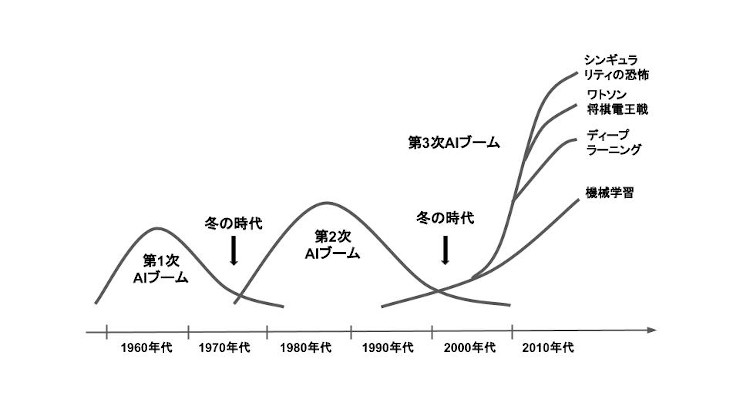
\includegraphics[clip, height=8cm, bb=10 0 160 104]{data/figure/ai_hist.jpg}
		\caption{AIのブームと冬の時代}
		\label{ai_hist_jpg}
	\end{center}
\end{figure}

Deep Learningが最初に脚光を浴びたのは,画像認識コンテスト ILSVRC(IMAGENET Large Scale Visual Recognition Challenge) \cite{overview_ilsvrc}で,2012年に2011年の優勝モデルのエラー率を約10\%下げて優勝した \cite{dl_hist4}.以降,Deep Learningを活用したアルゴリズムが台頭し,2015年には,人間のエラー率5.1\% \cite{arxiv_ilsvrc}を下回るアルゴリズムが登場した\footnote{図\ref{ilsvrc_winner_2010-2016}の引用元のAINOWが何を参照して人間のエラー率を4\%と定義したのかは不明} (図\ref{ilsvrc_winner_2010-2016}, 図\ref{ilsvrc_human_classification_results}).

\begin{figure} [H]
	\begin{center}
		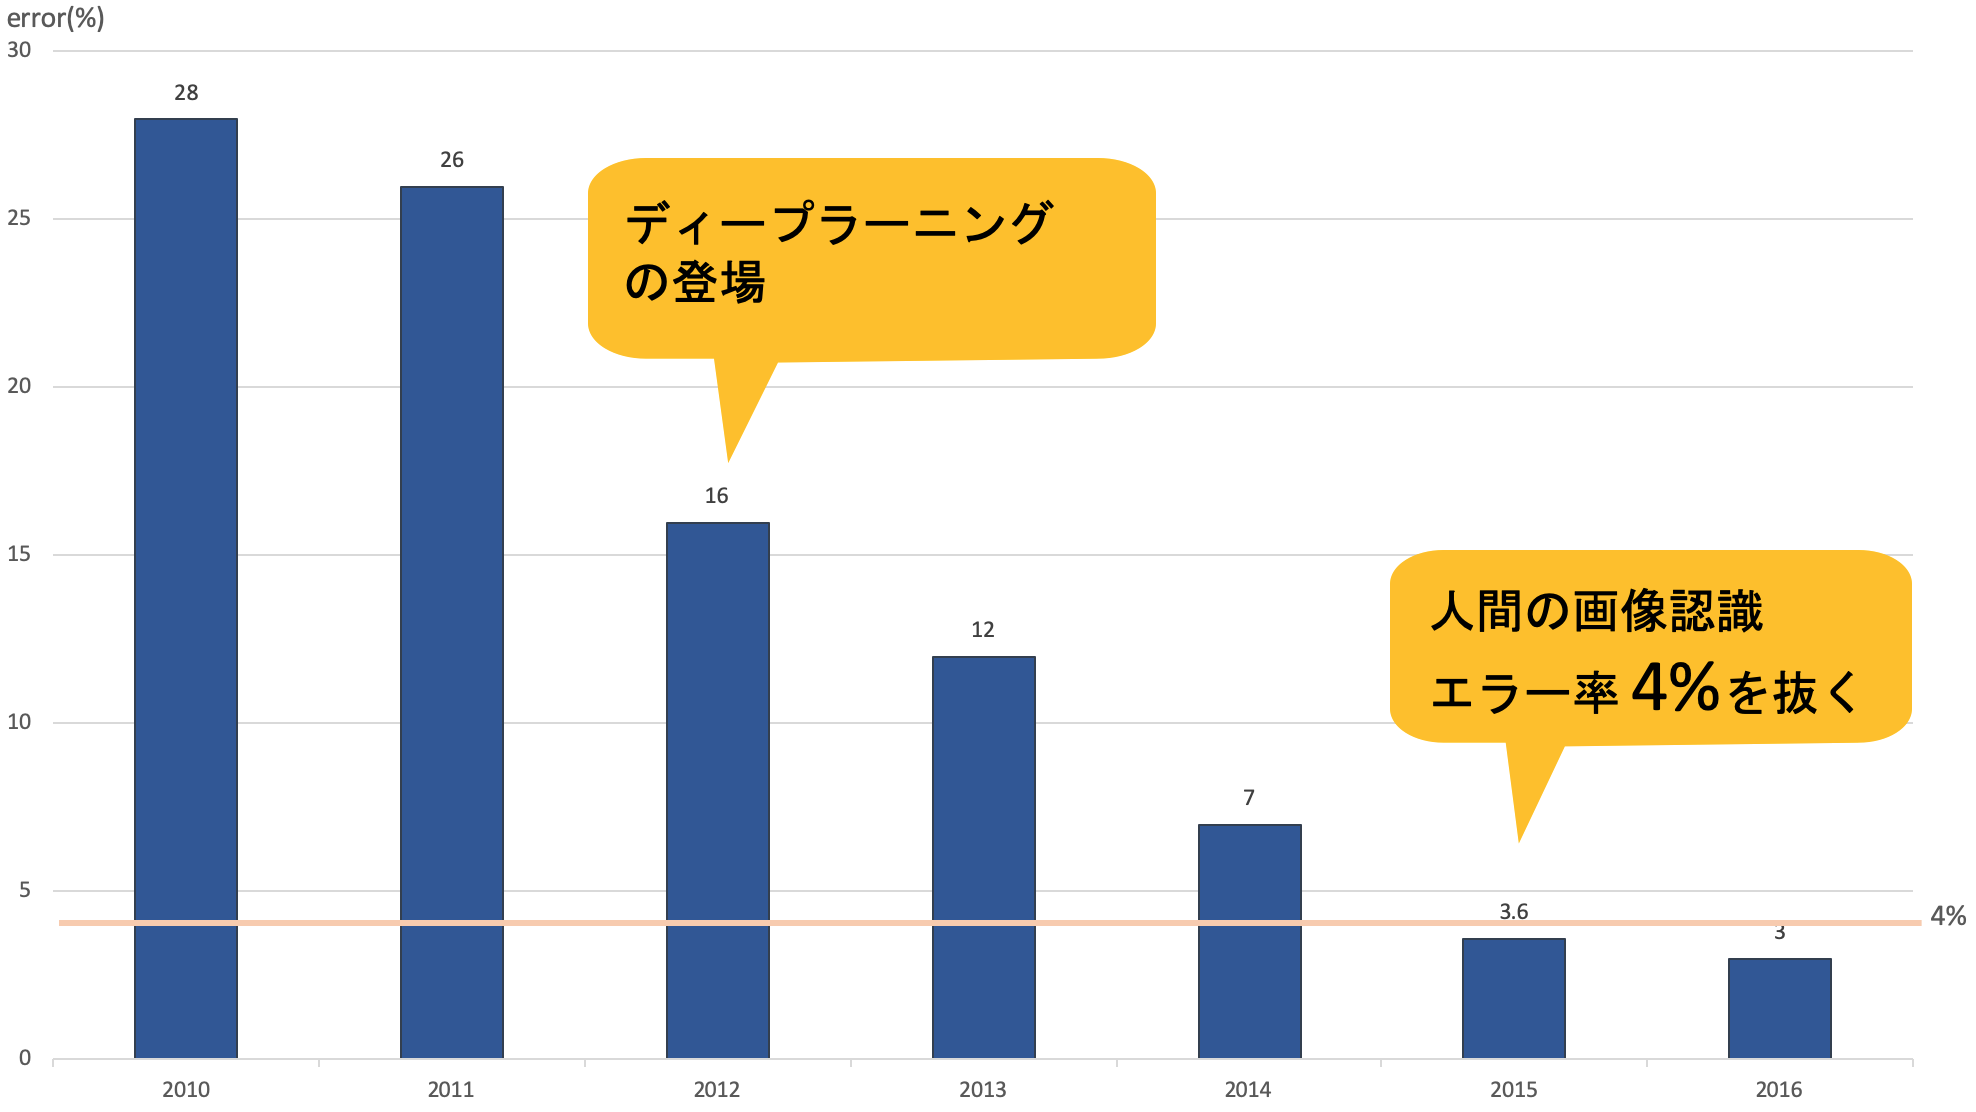
\includegraphics[clip, height=6cm, bb=0 0 1976 1112]{data/figure/ilsvrc_winner_2010-2016.png}
		\caption{ILSVRCの歴代優勝モデル(2010年~2016年)}
		\label{ilsvrc_winner_2010-2016}
	\end{center}
\end{figure}

\begin{figure} [H]
	\begin{center}
		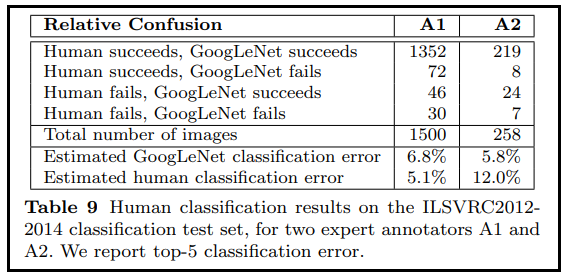
\includegraphics[clip, height=6cm, bb=-120 0 568 278]{data/figure/ilsvrc_human_classification_results.png}
		\caption{人間の画像認識エラー率}
		\label{ilsvrc_human_classification_results}
	\end{center}
\end{figure}文字認識

2012年以降のILSVRCの優勝モデルは,図\ref{ilsvrc_winner_2010-2017_with_algo}に示す通り \cite{dl_hist6} \footnote{図中,2014年の優勝モデルはGooLeNetとなっているが,正しくはGoogLeNet}.

\begin{figure} [H]
	\begin{center}
		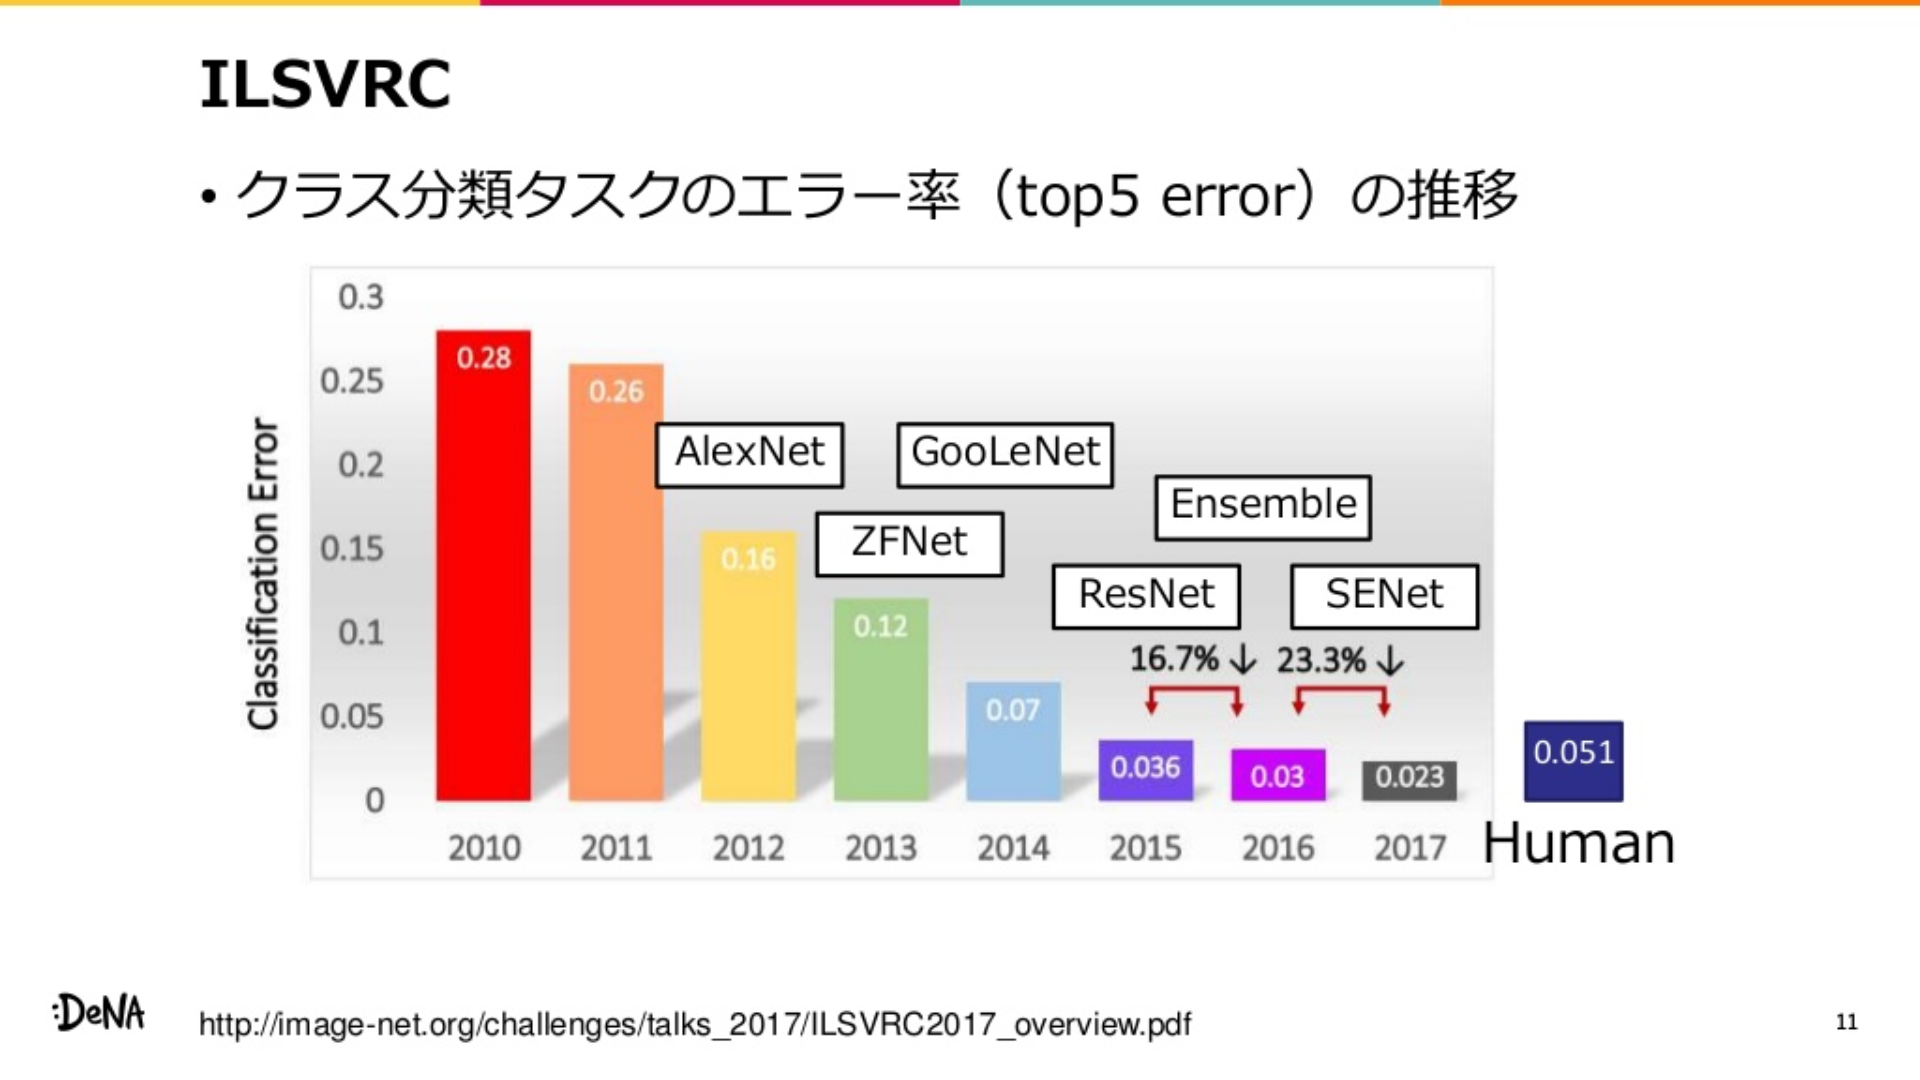
\includegraphics[clip, height=9cm, bb=-200 0 1920 1080]{data/figure/ilsvrc_winner_2010-2017_with_algo.png}
		\caption{2012年以降の優勝モデル}
		\label{ilsvrc_winner_2010-2017_with_algo}
	\end{center}
\end{figure}
